\documentclass{article}
\usepackage{tikz}
\usetikzlibrary{external}
\tikzexternalize

\usepackage{minted}
\usemintedstyle{one-dark}

\usepackage{booktabs}

\newmintinline[mono]{}{breakanywhere}
\newminted{python}{breakanywhere,tabsize=2,autogobble,breaklines=true, escapeinside=||}
\newenvironment{monos}{\VerbatimEnvironment\begin{pythoncode}}{\end{pythoncode}}

\begin{document}
\section{Overview}

\begin{itemize}
    \item Automatic mean of testing effectiveness of current model (\textbf{MSE} or
          \textbf{loss}).
    \item Automatic mean to improve/altering the weight assignment so as to
          optimize the model (\textbf{backpropagation} or \textbf{stochastic gradient descent}).
    \item Learn from experience.
\end{itemize}

\begin{figure}[htb]
    \centering
    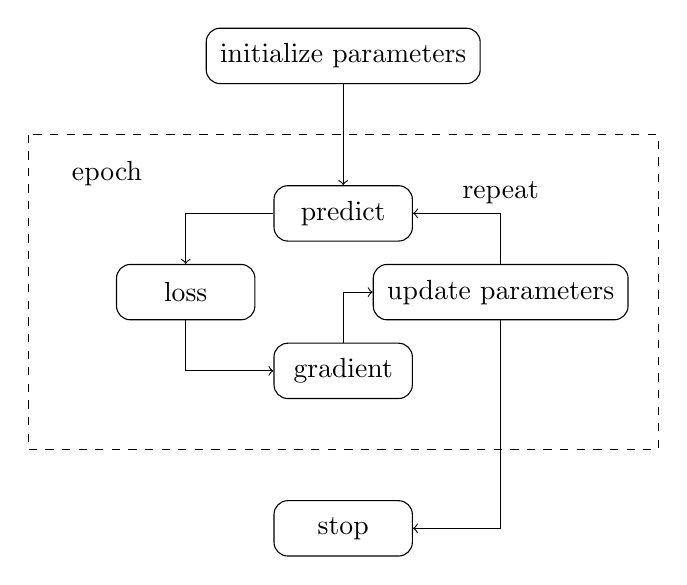
\begin{tikzpicture}[sibling distance=80pt, box/.style={rectangle, rounded corners=5pt, minimum width=50pt, minimum height=20pt, inner sep=5pt, draw}]
        \node[box] (init) at (0,1) {initialize parameters};
        \node[box] (pred) at (0,-1) {predict};
        \node[box] (loss) at (-2,-2) {loss};
        \node[box] (update) at (2,-2) {update parameters};
        \node[box] (grad) at (0,-3) {gradient};
        \node[box] (stop) at (0,-5) {stop};

        \draw[dashed] (-4, 0) rectangle (4, -4);
        \node at (-3.0, -0.5) {epoch};

        \draw[->] (init) -- (pred);
        \draw[->] (pred) -| (loss);
        \draw[->] (loss) |- (grad);
        \draw[->] (grad) |- (update);
        \draw[->] (update)  |- node[anchor=south] {repeat}  (pred);
        \draw[->] (update) |- (stop);

    \end{tikzpicture}
    \caption{The gradient descent process}
    \label{fig:gradient_descent}
\end{figure}

\begin{description}
    \item[Initialize parameters] Initialize all the parameters to random values.
    \item[Loss] the way of testing the effectiveness of the model (current weight
        assignment). Return a number, which smaller the number, the better the performance
        (by convention).
    \item[Update parameters] Update the parameters according to the gradient (which
        save us from trying each parameter in 2 directions).
    \item[Stop] When we finished our training (enough epoch that we decided has
        passed / the accuracy of the model started getting worse/ran out of time).
\end{description}

\subsection{Gradients}

The gradients point to the direction in which the function changes the most, which will tell us
how much do we have to change each weight to make our model better -- calculus is used
here to reduce the calculation.

Since our function has a lot of weights that we need to adjust, a lot of derivatives
(gradient) will be yielded.

We will use PyTorch to calculate the gradient.

\begin{enumerate}
    \item Tagging the variable that we want to calculate the gradient of it.
          \begin{monos}
              xt = tensor().requires_grad_()
          \end{monos}
    \item This tensor will contain a \verb!grad_fn! property, which will be used to calculate the gradient.
          \begin{monos}
              yt = f(xt)
          \end{monos}
    \item Calculate the gradient of \verb!yt! with respect to \verb!xt!. Refer to backpropagation.
          \begin{monos}
              yt.backward()
          \end{monos}
    \item The gradient of \verb!yt! with respect to \verb!xt! is stored in \verb!xt.grad!.
          \begin{monos}
              xt.grad
          \end{monos}
\end{enumerate}

Because of broadcasting, we can calculate the gradient of multiple variables at once
(i.e., build a large tensor and do the same thing).

Gradient only provides the slope of our function -- by timing the slope with a
\textit{learning rate}(IR), we can adjust the weight to make our model better (i.e.,
adjust weight proportionally to the gradient). IR is usually between 0.001 and 0.1, and
it could be anything.

We will use the learning rate finder to find the best learning rate. Adjust the weight by that
\begin{monos}
    w -= w.grad * lr
\end{monos}
will make our model gradually optimize and stick at the extremum.

Picking a learning rate that is too high would cause the function to bounce around and
never converge. Picking a learning rate that is too low would take a lot of time for it
to converge. Hence, we need to find a good learning rate. In this example, we will
stick with $1.0\times 10^{-4}$.

\section{Speed of Roller Coaster Example}

\begin{description}
    \item[Goal] We want to build a model that predicts the speed of a roller coaster as it went
        over the top of a hump.
    \item[Data] The model will take time as an independent variable, and predict the speed
        of the roller coaster as the dependent variable.
\end{description}

\subsection{Generate Data}

\begin{monos}
    time = torch.arange(0, 20).float()
    speed = torch.randn(20) * 3 + 0.75 * (time - 9.5) ** 2 + 1
\end{monos}

\begin{figure}[H]
    \centering
    \includegraphics[width=0.8\textwidth]{assets/generated_data.png}
    \caption{Generated data}
\end{figure}

\subsection{Quadratic Model}

\begin{monos}
def f(t, params):
    a, b, c = params
    return t ** 2 * a + b * t + c
\end{monos}

\subsection{Loss Function}

\begin{monos}
def mse(preds, targets):
    return ((preds - targets) ** 2).mean()
\end{monos}

\subsection{Initialize weights}

\begin{monos}
def init_params(shape):
    return torch.randn(shape).requires_grad_()
params = init_params(3)
\end{monos}

\subsection{Prediction}

\begin{monos}
def show_preds(preds, ax=None):
    if ax is None:
        _, ax = plt.subplots()
    ax.scatter(time, speed, label="label")
    ax.scatter(time, to_np(preds), color="red", label="pred")
    ax.legend()
    ax.set_ylim(-300, 100)
\end{monos}

\subsection{Gradient}

\begin{monos}
def cal_grad(loss):
    loss.backward()
    return params.grad.data
\end{monos}

\subsection{Adjustment \& LR}

\begin{monos}
lr = 1e-5

def adjust(grad):
    params.data -= grad * lr
    params.grad = None

def epoch():
    preds = f(time, params)
    loss = F.mse_loss(preds, speed)
    adjust(grad := cal_grad(loss))
    return grad
\end{monos}

\subsection{Epoch \& Repeat}

\begin{monos}
for _ in range(10):
    epoch()

show_preds(f(time, params.data))
\end{monos}

\begin{figure}[H]
    \centering
    \includegraphics[width=0.8\textwidth]{assets/model.png}
    \caption{Predicted Result}
\end{figure}

\section{MNIST}

\begin{description}
    \item[Goal] We want to build a model that can predict the digit of an MNIST image.
    \item[Data] Image and their corresponding digit.
\end{description}

\subsection{Prepare Data}

\begin{monos}
path = untar_data(URLs.MNIST_SAMPLE)
data = (
    lambda type, label: torch.stack(
        [tensor(Image.open(img)) for img in (path / type / label).ls()]
    )
    / 255.0
)
xy = (
    lambda type: (torch.cat(d := [data(type, lbl) for lbl in "37"]).view(-1, 28 * 28),
    tensor([1] * len(d[0]) + [0] * len(d[1])).unsqueeze(1))
)
train_x, train_y = xy("train")
valid_x, valid_y = xy("valid")
\end{monos}

\subsection{Initialize}

\begin{monos}
def init_weights(size, std = 1.0):
    return (torch.randn(size) * std).requires_grad_()
# y = w * x + b
weights = init_weights((28 * 28, 1))
bias = init_weights(1)
\end{monos}

\subsection{Model}

\begin{monos}
# y = w * x + b
def pred(xb):
    return xb @ weights + bias
\end{monos}

\subsection{Loss \& Metric}

\begin{monos}
def accuracy(pred, yb):
    """
    Metric that drives our understanding. 
    
    Not suitable for AI, since a small weight change won't change accuracy at all. 
    Hence, it is useless as a loss function -- it only yields two gradients: infinite or 0.
    """
    return ((pred > 0.0).float() == yb).float().mean().item()


def mnist_loss(prds, trgts):
    """
    Loss function that is used to drive AI.

    Sensitive to small changes. 
    Loss function needs to be smooth and consistent/small derivative everywhere.
    """
    # Activiation function. Ensure prds between [0, 1]. lambda sigmoid: 1/(1 + torch.exp(-x))
    prds = prds.sigmoid()
    # Equiv: [b[i] if e else c[i] for i, e in enumerate(a)]
    return torch.where(trgts == 1, 1 - prds, prds).mean()
\end{monos}

\subsection{Mini Batcher}

\begin{monos}
# y = w * x + b
def pred(xb):
    return xb @ weights + bias
\end{monos}

\subsection{Gradient}

\begin{monos}
def calc_grad(xb, yb):
    prds = pred(xb)
    loss = mnist_loss(prds, yb)
    loss.backward()
\end{monos}

\subsection{Adjustment \& LR}

\begin{monos}
def calc_grad(xb, yb):
    prds = pred(xb)
    loss = mnist_loss(prds, yb)
    loss.backward()

params = weights, bias
for epoch in range(20):
    train_epoch(params)
    print(f"{epoch:-5} | {validate_epoch():.2f}")
\end{monos}

\section{Optimizer}

SGD is a very general optimization algorithm. Hence, PyTorch provided useful classes to
make it easier to implement.

\subsection{Linear Model}

\begin{monos}
    linear_model = nn.Linear(28 * 28,  1)
    weights, bias = linear_model.parameters()
\end{monos}

\subsection{Optimizer}

\begin{monos}
    class BasicOptim:
    def __init__(self, params, lr):
        self.params = list(params)
        self.lr = lr
    def step(self, *args, **kwargs):
        for p in self.params:
            p.data -= p.grad.data * self.lr
    def zero_grad(self, *args, **kwargs):
        for p in self.params:
            p.grad = None
    opt = BasicOptim(linear_model.parameters(), lr)
\end{monos}

\subsection{Train}

\begin{monos}
    def train_epoch(model):
    for xb, yb in dl:
        calc_grad(xb, yb, model)
        opt.step()
        opt.zero_grad()


def train_model(model, epochs):
    for i in range(epochs):
        train_epoch(model)
        print(validate_epoch(model), end=" ")


train_model(linear_model, 20)
\end{monos}

\section{Fastai SGD}

\begin{monos}
linear_model = nn.Linear(28 * 28, 1)
opt = SGD(linear_model.parameters(), lr)
train_model(linear_model, 20)
\end{monos}

In addition to SGD, Fastai also provides \verb!Learn.fit!, which can be called with
\verb!train_model! directly

\begin{monos}
dls = DataLoaders(train_dl, valid_dl)
learn = Learner(
    dls,
    nn.Linear(28 * 28, 1),
    opt_func=SGD,
    loss_func=mnist_loss,
    metrics=accuracy,
)
learn.fit(10, lr=lr)
\end{monos}

\section{Nueral Network}

We have a linear classifier, but it is not enough. We need to add more layers in order
for it to do anything more complex than just classify 3 and 7.

\subsection{Overview}

\begin{monos}
def simple_net(xb):
    res = xb @ w1 + b1
    res = res.max(tensor(0.0))
    res = res @ w2 + b2
    return res
\end{monos}

A neural net is defined as a bunch of linear models that connect each layer to the next
with a \verb!max! function. This function is rectified linear unit also known as
\textit{ReLU} and formally defined by $\textrm{ReLU}(x) = max(x, 0)$.

The rectified linear unit function is the key: if we just put linear layers one after
each other, then there is no difference between using multiple of them or just one
(composition of linear functions is another linear function).

\textit{Universal approximation theorem}: with enough amount of small pieces of linear
function, one would be able to approximate any function to any accuracy desired.

\begin{monos}
simple_net = nn.Sequential(
    nn.Linear(28 * 28, 30),
    nn.ReLU(),
    nn.Linear(30, 1),
)
learn = Learner(
    dls,
    simple_net,
    opt_func=SGD,
    loss_func=mnist_loss,
    metrics=accuracy,
)
# Because this is a deeper model, we will use a smaller learning rate.
learn.fit(40, lr=0.1)
\end{monos}

At this point, we have a model that can classify 3 and 7 at the accuracy of 98.28\%; As
well as two magic algorithms:

\begin{itemize}
    \item A function which solves any problem to any level of accuracy.
    \item A algorithm which finds the best set of parameters of any function (minimize
          loss).
\end{itemize}

\section{Deeper}

\begin{itemize}
    \item As the model gets deeper, it becomes harder to train and optimize.
    \item A deeper model, which uses smaller matrices with more layers compared to a
          shallower model, gets a better result and is faster in production.
\end{itemize}

\section{Summary}

\begin{description}
    \item[Activations] Numbers that are calculated from the model.
    \item[Parameters] Numbers that are randomly initialized and optimized.
    \item[Tensor] A regularly shaped array. Activations and parameters are all stored
        in a tensor.
        \begin{description}
            \item[Axes] Dimensions of the tensor \verb!tensor.shape!.
            \item[Rank] Number of axes \verb!tensor.ndim!.
                \begin{description}
                    \item[Scalar] rank 0 tensor.
                    \item[Vector] rank 1 tensor.
                    \item[Matrix] rank 2 tensor.
                \end{description}
        \end{description}
    \item[Layer] linear or nonlinear function which takes inputs from the previous layer and
        produces outputs by repetitively applying the function.
    \item[ReLU] Rectified linear unit function, \verb!lambda x: max(x, 0)!
    \item[Mini-Batch] A small group of inputs and labels gathered together in two
        arrays. A gradient descent step is updated on this batch (rather than a whole data
        set, as it would be time-consuming and expensive without sacrificing a lot of
        information).
    \item[Gradient] The derivative of the loss function of all the parameters.
    \item[Loss] A value that represents how well/bad the model is doing.
    \item[Backward pass] Computing the gradient of the loss function for
        all model parameters.
    \item[Gradient Descent] A method of updating the parameters of a model by taking a
        step in the direction opposite to the gradient (so it would reach local min/max).
    \item[Forward Pass] Applying the model to some input and computing the predictions.
    \item[Learning Rate] The size of the step taken in the gradient descent.
\end{description}

\end{document}